\section{Method}
\label{sec:method}

\method\ is a channel-independent linear forecaster built from three components:
(i) a learnable, lossless frequency decomposition that routes the input into $K$
bands (Section~\ref{sec:method:freq}); (ii) one lightweight linear head per band
followed by recombination (Section~\ref{sec:method:heads}); and (iii) Adaptive
Reversible Instance Normalization (\arevin), a \emph{regime-adaptive} reversible
normalization that strictly generalizes RevIN \citep{kim2022revin}
(Section~\ref{sec:method:arevin}). Throughout, the design is deliberately
minimal: every added component is an opt-in generalization of a known linear
baseline, and each degenerates back to that baseline when its parameters take
their identity values. This yields the strict nesting
$\text{Linear} \subseteq \text{RLinear} \subseteq \method$, which forms the
backbone of the ablation study (Section~\ref{sec:ablation}).

\subsection{Problem Setup and Notation}
\label{sec:method:setup}

We observe a multivariate lookback window
$\bX \in \R^{B \times L \times C}$ of length $L$ over $C$ variates (channels)
and predict the future horizon $\bY \in \R^{B \times H \times C}$ of length
$H$, where $B$ is the batch size. Following the strong-baseline convention of
DLinear \citep{zeng2023dlinear}, RLinear \citep{li2023rlinear} and PatchTST
\citep{nie2023patchtst}, \method\ is \emph{channel-independent} (CI): every
variate is processed by the \emph{same} shared weights, and the channel
dimension is folded into the batch. Concretely, we reshape
$\bX : B{\times}L{\times}C \to (B{\cdot}C){\times}L$, operate on
$N = B{\cdot}C$ univariate series of length $L$, and reshape predictions back
to $B{\times}H{\times}C$. CI keeps the parameter count independent of $C$,
which is essential for the 4\,GB memory budget and for high-dimensional
datasets such as Electricity ($C{=}321$). Unless a tensor shape indicates
otherwise, the equations below are written for a single univariate series
$\bs \in \R^{L}$.

We use the real FFT throughout: \texttt{rfft}/\texttt{irfft} along the time
axis. For a real length-$L$ signal, \texttt{rfft} returns
$F = \lfloor L/2 \rfloor + 1$ non-redundant complex bins, and
$\texttt{irfft}(\cdot, n{=}L)$ inverts it exactly. All transforms are of length
$L$ (the lookback); the model never applies an FFT to the horizon. The default
and primary number of bands is $K{=}2$ (a low and a high band); $K \in \{3,4\}$
is explored only as an ablation.

Figure~\ref{fig:arch} gives the end-to-end forward pass: \arevin\ normalization,
the learnable frequency split, per-band linear heads, additive recombination,
and \arevin\ denormalization.

\begin{figure}[t]
  \centering
  \IfFileExists{../results/figures/architecture.pdf}{%
    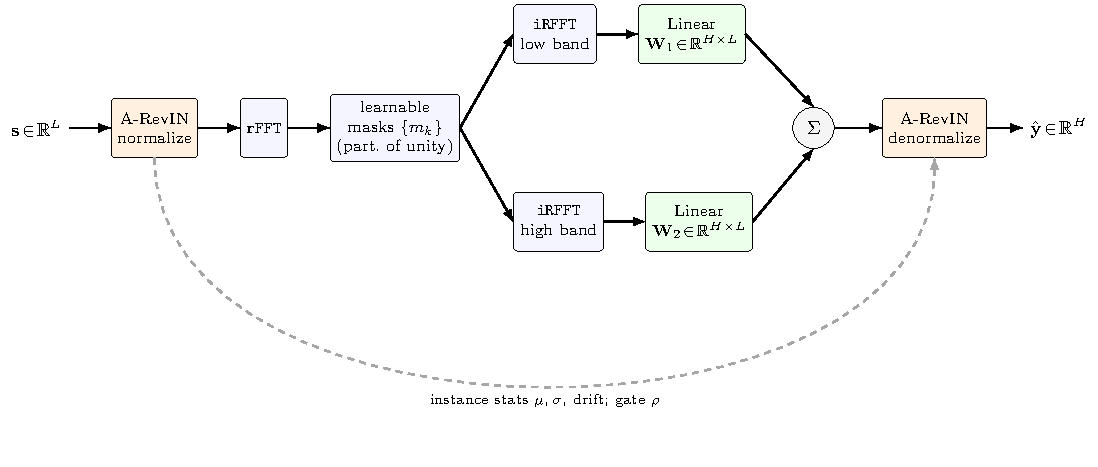
\includegraphics[width=\linewidth]{../results/figures/architecture.pdf}%
  }{\fbox{\parbox[c][0.18\textheight][c]{0.9\linewidth}{\centering
    \textbf{[architecture figure pending]}}}}
  \caption{Overview of the \method\ forward pass for one channel-independent
  series. A-RevIN normalizes the input and stores its instance statistics; a
  learnable partition-of-unity spectral filter splits the normalized series into
  $K$ bands; each band is forecast by a dedicated linear head; the band
  forecasts are summed and de-normalized by the horizon-adaptive A-RevIN
  inverse.}
  \label{fig:arch}
\end{figure}

\subsection{Adaptive Reversible Instance Normalization (\arevin)}
\label{sec:method:arevin}

RevIN \citep{kim2022revin} normalizes each instance by its own lookback
mean/standard deviation, applies an optional affine transform, runs the model,
and then inverts the affine and re-applies the stored statistics. Its known
weakness is that it de-normalizes the \emph{entire} horizon with the
\emph{single} lookback statistic pair $(\mu, \sigma)$: under non-stationarity,
the horizon's true level and scale drift away from the lookback statistics, and
the error grows with horizon distance. \arevin\ retains RevIN's reversible
structure but makes the de-normalization \emph{horizon-adaptive} and
\emph{gated}, so that RevIN is recovered exactly as a special case.

\paragraph{Normalization (identical to RevIN).}
For a series $\bs \in \R^{L}$, statistics are taken over the time axis:
\begin{align}
\mu &= \frac{1}{L}\sum_{i=1}^{L} s_i, &
\sigma &= \sqrt{\tfrac{1}{L}\sum_{i=1}^{L}(s_i - \mu)^2 + \epsilon}, \\
\tilde{s}_i &= \frac{s_i - \mu}{\sigma}, &
s^{\mathrm{n}}_i &= \gamma\,\tilde{s}_i + \beta,
\label{eq:revin-norm}
\end{align}
with stabilizer $\epsilon = 10^{-5}$. The affine parameters
$\gamma, \beta \in \R$ are \emph{scalars} shared across all series and channels;
this preserves channel independence and keeps the parameter count independent of
$C$ (standard RevIN uses per-channel affine vectors of size $C$).

\paragraph{Adaptive de-normalization.}
Let $\bp \in \R^{H}$ be the band-recombined prediction in the normalized space
(Section~\ref{sec:method:heads}). Standard RevIN inverts every horizon step
$t \in \{1,\dots,H\}$ identically as
$\hat{y}_t = \sigma\,(p_t - \beta)/\gamma + \mu$. \arevin\ introduces three
learnable per-step vectors and one gate:
\begin{equation}
\mathbf{a} \in \R^{H},\quad
\mathbf{b} \in \R^{H},\quad
\boldsymbol{\lambda} \in \R^{H},\quad
\rho = \varsigma(r) \in (0,1),
\label{eq:arevin-params}
\end{equation}
where $\mathbf{a}$ is a per-step log-scale correction (initialized
$\mathbf{a}{=}\mathbf{0}$, so $\exp(0){=}1$), $\mathbf{b}$ is a per-step shift
correction in units of $\sigma$ (initialized $\mathbf{0}$),
$\boldsymbol{\lambda}$ is a per-step drift-propagation coefficient (initialized
$\mathbf{0}$), $\varsigma$ is the logistic sigmoid, and $\rho$ is a scalar gate
obtained from a raw parameter $r$. The initialization of $r$ is consequential and
is discussed below. We also compute a non-learnable \emph{drift} feature from
detached lookback statistics, capturing the recent-versus-early level change in
units of $\sigma$:
\begin{equation}
\mathrm{drift} =
\frac{\operatorname{mean}\!\big(\bs_{L/2:L}\big)
      - \operatorname{mean}\!\big(\bs_{0:L/2}\big)}{\sigma}.
\label{eq:drift}
\end{equation}
The horizon-adaptive inverse, applied per step $t = 1,\dots,H$, is
\begin{align}
\mathrm{scale}_t &= \exp\!\big(\rho\, a_t\big), \label{eq:arevin-scale}\\
\mathrm{shift}_t &= \rho\,\big(b_t\,\sigma + \lambda_t\,\mathrm{drift}\,\sigma\big),
  \label{eq:arevin-shift}\\
\hat{y}_t &= \mathrm{scale}_t \cdot
  \Big[\sigma\,\frac{p_t - \beta}{\gamma}\Big] + \mu + \mathrm{shift}_t.
  \label{eq:arevin-denorm}
\end{align}
The $\lambda_t$ term lets the model propagate the \emph{observed} lookback drift
into the horizon proportionally to step distance, providing a horizon-aware
extrapolation of level: $\lambda_t$ is expected to grow with $t$ on trending
datasets and to stay near zero on stationary ones.

\paragraph{Reversibility and identity guarantee.}
When $\rho = 0$ (equivalently
$\mathbf{a}=\mathbf{b}=\boldsymbol{\lambda}=\mathbf{0}$),
Equations~\eqref{eq:arevin-scale}--\eqref{eq:arevin-denorm} reduce \emph{exactly}
to the RevIN inverse $\hat{y}_t = \sigma\,(p_t-\beta)/\gamma + \mu$. Hence
$\text{RevIN} \subset \arevin$: training cannot do worse than RevIN at the
normalization layer up to optimization, and the gate $\rho$ lets the model learn
to stay at RevIN when adaptation does not help---making \arevin\
\emph{regime-adaptive}: it can engage where adaptation helps and reduce to RevIN
where it does not. \arevin\ adds $3H+3$ parameters
($\gamma,\beta,r$ plus $\mathbf{a},\mathbf{b},\boldsymbol{\lambda}$); for
$H{=}720$ this is $2163$ parameters, all shared across channels.

\paragraph{Gate initialization and a gradient trap.}
The reversibility guarantee makes a small gate value at initialization tempting,
but it conceals a gradient trap. Because the adaptive parameters start at their
identity values ($\mathbf{a}=\mathbf{b}=\boldsymbol{\lambda}=\mathbf{0}$), the
per-step corrections in
Equations~\eqref{eq:arevin-scale}--\eqref{eq:arevin-shift} are exactly zero at
initialization regardless of $\rho$, so $\partial\mathcal{L}/\partial\rho \approx
0$ and the gate receives essentially no gradient signal. Initializing $r$ so that
$\rho \approx 0$ therefore leaves \arevin\ dormant at RevIN throughout training,
even on data where adaptation would help. We instead initialize $r{=}0$ (so
$\rho{=}0.5$), which gives the gate a non-zero gradient and lets it open or close
as the data dictates; this is our default. Note that RevIN is still recovered
\emph{exactly} at the learned value $\rho{=}0$, so this initialization does not
compromise the identity guarantee---it only ensures the gate is trainable. We
quantify the effect of this choice in Section~\ref{sec:results:nonstat}.

\paragraph{Scope.}
\arevin\ is a \emph{first-order}, horizon-aware level/scale correction: it does
not model full distributional shift (there is no per-step variance modeling
beyond the scalar $\exp(\rho\,a_t)$), and the drift feature in
Equation~\eqref{eq:drift} is a simple two-half mean difference rather than a
learned encoder. This is deliberate, keeping \arevin\ at linear-model cost and
interpretable, and positioning it as a lightweight counterpart to heavier
stationarity-aware methods such as Non-stationary Transformers
\citep{liu2022nonstationary}.

\subsection{Learnable Frequency Decomposition}
\label{sec:method:freq}

DLinear \citep{zeng2023dlinear} decomposes a series into trend and seasonal
components using a \emph{fixed} moving-average kernel, i.e. a fixed-width
low-pass / high-pass split in the time domain. \method\ makes this split
\emph{learnable in the frequency domain} with a smooth, monotone,
parameter-light soft mask, and generalizes it from two bands to $K$. This is a
modest, defensible generalization of DLinear's decomposition; we explicitly do
\emph{not} claim to be the first frequency-domain linear forecaster
(cf. FEDformer \citep{zhou2022fedformer}, FiLM \citep{zhou2022film}, FreTS
\citep{yi2023frets}, and especially FITS \citep{xu2024fits}).

\paragraph{Soft spectral masks.}
Let the normalized frequency of rfft bin $f \in \{0,\dots,F-1\}$ be
\begin{equation}
\omega_f = \frac{f}{F-1} \in [0,1],
\qquad \omega_0 = 0\ (\text{DC}),\quad \omega_{F-1} = 1\ (\text{Nyquist}).
\end{equation}
For the primary case $K{=}2$ we learn a raw cutoff $c \in \R$ and a raw
sharpness $\tau \in \R$, and form
\begin{align}
\mathrm{cutoff} &= \varsigma(c) \in (0,1), &
\mathrm{sharpness} &= \operatorname{softplus}(\tau) + \epsilon_m \in (0,\infty),
\end{align}
with $\epsilon_m = 10^{-3}$, and define complementary low- and high-pass masks
\begin{align}
m_{\mathrm{low}}(\omega_f) &= \varsigma\!\big(-\,\mathrm{sharpness}\cdot(\omega_f - \mathrm{cutoff})\big),
  \label{eq:mask-low}\\
m_{\mathrm{high}}(\omega_f) &= 1 - m_{\mathrm{low}}(\omega_f).
  \label{eq:mask-high}
\end{align}
Here $m_{\mathrm{low}}$ is a smooth monotone-decreasing low-pass filter and
$m_{\mathrm{high}}$ is its exact complement, so the masks form a
\emph{partition of unity}: $\sum_k m_k(\omega_f) = 1$ for every bin. For general
$K$, we use $K-1$ ordered cutoffs $0 < c_1 < \dots < c_{K-1} < 1$ (ordering
enforced by a cumulative-softplus parameterization) and define
\begin{align}
m_1 &= \varsigma\!\big(-\tau_1(\omega - c_1)\big), \nonumber\\
m_k &= \varsigma\!\big(-\tau_k(\omega - c_k)\big)
       - \varsigma\!\big(-\tau_{k-1}(\omega - c_{k-1})\big),
       \quad 1 < k < K, \label{eq:mask-general}\\
m_K &= 1 - \varsigma\!\big(-\tau_{K-1}(\omega - c_{K-1})\big), \nonumber
\end{align}
which again partition unity by construction.

\paragraph{Application to the spectrum.}
The masks $m_k \in \R^{F}$ are real-valued and multiply the complex spectrum
bin-wise (the same real scalar scales the real and imaginary parts, so phase is
preserved and the gating is pure magnitude):
\begin{align}
\mathbf{S} &= \texttt{rfft}(\bs^{\mathrm{n}}, n{=}L), &
\mathbf{S}^{(k)} &= m_k \odot \mathbf{S}, &
\bs^{\mathrm{n},(k)} &= \texttt{irfft}\big(\mathbf{S}^{(k)}, n{=}L\big),
\label{eq:band-split}
\end{align}
where $\mathbf{S}, \mathbf{S}^{(k)} \in \mathbb{C}^{F}$ and
$\bs^{\mathrm{n},(k)} \in \R^{L}$. The masks depend only on the learnable scalars
(recomputed cheaply each forward pass) and are independent of both the batch and
the channel.

\paragraph{Properties.}
The decomposition has four properties that make it defensible:
(1)~\emph{Lossless partition}: since $\sum_k m_k = 1$ exactly,
$\sum_k \bs^{\mathrm{n},(k)} = \texttt{irfft}\big(\sum_k m_k \odot \mathbf{S}\big)
= \texttt{irfft}(\mathbf{S}) = \bs^{\mathrm{n}}$, so reconstruction is exact
\emph{before} the heads.
(2)~\emph{DLinear as a special case}: with $K{=}2$ and
$\mathrm{sharpness}\to\infty$, the soft mask approaches an ideal low/high split,
recovering the trend/residual inductive bias of DLinear's fixed box filter as one
member of a strictly richer, learnable family.
(3)~\emph{Differentiability}: $\mathrm{cutoff}$ and $\mathrm{sharpness}$ receive
gradients through \texttt{irfft}, so the split adapts to each dataset's spectral
content during training.
(4)~\emph{Cheapness}: the decomposition adds only $2(K-1)$ scalar parameters,
and the FFT/iFFT cost is $O(L\log L)$ per series, negligible relative to the
$H{\cdot}L$ linear heads.

\paragraph{Contrast with FITS.}
FITS \citep{xu2024fits}, the closest prior art, applies a low-pass cutoff in the
rFFT domain and forecasts with a single complex linear layer, thereby
\emph{discarding} all high-frequency content above the cutoff. \method's split is
different in kind: it is a partition of unity that \emph{keeps} all frequency
content and routes each band to its own dedicated head, so the high-frequency
band is \emph{modeled} rather than thrown away. This is a falsifiable difference
that the ablation in Section~\ref{sec:ablation} tests directly; if the spectral
split adds little over RLinear once \arevin\ is present, we report that plainly.

\paragraph{Initialization.}
For $K{=}2$ we initialize $\mathrm{cutoff}\approx 0.25$
(raw $c = \operatorname{logit}(0.25) \approx -1.0986$), so the low band starts as
roughly the lowest quarter of frequencies (a trend / low-season prior), and
$\mathrm{sharpness}\approx 10$. These are starting points and are subsequently
learned; we assert $0.02 < \mathrm{cutoff} < 0.98$ at initialization to avoid a
degenerate all-pass or all-stop mask, and we report the final learned values per
dataset as an interpretability artifact.

\subsection{Per-Band Linear Heads and Recombination}
\label{sec:method:heads}

\paragraph{Heads.}
Each band is forecast by one independent linear head mapping the lookback length
$L$ to the horizon length $H$:
\begin{equation}
\bp^{(k)} = \mathbf{W}_k\, \bs^{\mathrm{n},(k)} + \mathbf{b}_k,
\qquad \mathbf{W}_k \in \R^{H \times L},\ \mathbf{b}_k \in \R^{H},
\label{eq:head}
\end{equation}
realized as a single \texttt{nn.Linear}$(L,H)$ with bias. Each head has
$H{\cdot}L + H$ parameters.

\paragraph{Recombination.}
The primary model uses an identity sum,
\begin{equation}
\bp = \sum_{k=1}^{K} \bp^{(k)} \in \R^{H}.
\label{eq:recomb}
\end{equation}
Because the bands sum to the input (lossless partition) and each head is linear,
the identity sum keeps the model in the same hypothesis class as a single linear
head while granting the ability to apply a \emph{different} linear map to
different frequency content---which is the entire point. In particular, with
$K{=}1$, an all-pass mask, and identity recombination, \method\ degenerates
exactly to RLinear (RevIN + Linear); this nesting underpins the ablation table.
As an ablation we also consider a learnable band gate $\mathbf{g}\in\R^{K}$ with
$\bp = \sum_k g_k\,\bp^{(k)}$, reported only if it helps and we can explain why.

\subsection{Complexity and Parameter Count}
\label{sec:method:complexity}

For the primary configuration $K{=}2$, the total parameter count is
\begin{equation}
\underbrace{2\,(H{\cdot}L + H)}_{\text{heads}}
+ \underbrace{2(K-1)}_{\text{decomposition}}
+ \underbrace{3H + 3}_{\arevin}
\;\approx\; 2HL + 5H + 5.
\label{eq:params}
\end{equation}
For $L{=}96, H{=}96$ this is $\approx 18.9$k parameters, and for
$L{=}336, H{=}720$ it is $\approx 487.5$k. By comparison, DLinear uses
$\approx 2HL$ and RLinear $\approx HL$, so \method\ is roughly twice the size of
a single linear head---still linear-scale and easily within the 4\,GB budget. We
report this $2\times$ parameter cost honestly: the claim is competitive or better
accuracy at still-linear scale, not a free improvement. The per-forward compute
is dominated by the $K$ matrix--vector products of the heads ($O(KHL)$ per
series), with the FFT/iFFT adding only $O(L\log L)$; we report exact analytic
FLOPs alongside measured train time and peak memory in
Section~\ref{sec:efficiency}.
